\appendix{Specyfikacja notacji LupN}\label{appendix:3}

Specyfikacja w formie elektronicznej znajduje się pod linkiem: \url{https://github.com/0x41gawor/lupus/blob/master/docs/spec/lupn.md}.


\hyperlink{def:lupn}{\textbf{LupN}} (od ang. \textit{loop} oraz \textit{Notation}) to język/notacja służąca do wyrażania \hyperlink{def:workflow-petli}{\textbf{Workflow Pętli}}. Nie zawiera opisu \hyperlink{def:czesc-obliczeniowa}{\textbf{Części Obliczeniowej}} \hyperlink{def:logika-petli}{\textbf{Logiki Pętli}}. \hyperlink{def:czesc-obliczeniowa}{\textbf{Część Obliczeniowa}} jest określona poza \hyperlink{def:lupus}{\textbf{Lupus}}, w \hyperlink{def:element-zewnetrzny}{\textbf{Elementach Zewnętrznych}}.

\texttt{LupN} specyfikuje:
\begin{itemize}
    \item \hyperlink{def:workflow-petli}{\textbf{Workflow Pętli}}, czyli workflow \hyperlink{def:element-lupus}{\textbf{Elementów Lupus}},
    \item odniesienia do \hyperlink{def:element-zewnetrzny}{\textbf{Elementów Zewnętrznych}}, wyrażone jako \hyperlink{def:destynacja}{\textbf{Destynacje}},
    \item \hyperlink{def:workflow-petli}{\textbf{Workflow Akcji}} w ramach \hyperlink{def:element-lupus}{\textbf{Elementu Lupus}},
    \item odniesienie (lub odniesienia) do \hyperlink{def:agent-egress}{\textbf{Agenta Egress}} jako \hyperlink{def:destynacja}{\textbf{Destynacja}}.
\end{itemize}

Jak można zauważyć, \texttt{LupN} wyraża \textbf{workflow} na dwóch poziomach: globalnym (czyli \hyperlink{def:workflow-petli}{\textbf{Workflow Elementów Lupus}}) oraz wewnątrz \hyperlink{def:element-lupus}{\textbf{Elementu Lupus}} (czyli \hyperlink{def:workflow-petli}{\textbf{Workflow Akcji}}). Możliwości obu poziomów są do siebie zbliżone, ale ostatecznie różne. Ten załącznik omówi również tę kwestię.


Z punktu widzenia implementacji \hyperlink{def:plik-lupn}{\textbf{Plik LupN}} to w rzeczywistości \textit{YAML manifest file} dla \hyperlink{def:zasoby-wlasne}{\textit{Zasobu Własnego}} \hyperlink{def:master}{\textbf{Master}}. Po zaaplikowaniu (ang. \textit{apply}), \hyperlink{def:operator-zasobu-master}{\textbf{Operator Zasobu Master}} uruchamia \hyperlink{def:element-lupus}{\textbf{Elementy Lupus}}, które realizują wyrażone \hyperlink{def:workflow-petli}{\textbf{Workflow Pętli}}.

\texttt{LupN} wyraża \hyperlink{def:workflow-petli}{\textbf{Workflow Pętli}} poprzez specyfikację różnych obiektów w notacji YAML. Nazwijmy te obiekty \hyperlink{def:obiekt-lupn}{\textbf{Obiektami LupN}}. \hyperref[appendix:3]{Załącznik 3} specyfikuje te obiekty oraz relacje między nimi. Wskazuje również, co oznacza użycie każdego z nich w kontekście \hyperlink{def:workflow-petli}{\textbf{Workflow Pętli}} i jak \hyperlink{def:operator-zasobu-element}{\textbf{Operator Zasobu Element}} je interpretuje w czasie działania.

Okazuje się, że obiekty YAML w \textbf{YAML manifest files} są pochodnymi struktur Golang (typów Golang), dlatego możemy opisać \hyperlink{def:obiekt-lupn}{\textbf{Obiekty LupN}} na podstawie tych struktur Golang. Obiekty YAML w \hyperlink{def:plik-lupn}{\textbf{Pliku LupN}} są pochodnymi struktur Go, dlatego \hyperlink{def:obiekt-lupn}{\textbf{Obiekty LupN}} możemy opisać na ich podstawie. 

Wymagane jest wcześniejsze zapoznanie się z YAML. Załącznik nie obejmuje translacji dokonywanej przez Kubernetes między strukturami Go a reprezentacjami obiektów YAML. Serializacja jest wykonywana przez \texttt{controller-gen} i opisana w \textit{Kubebuilder Book}. Tłumaczenie to można łatwo zaobserwować i nauczyć się, analizując przykłady zamieszczone w repozytorium projektu: \url{https://github.com/0x41gawor/lupus/tree/master/examples}

\subsection{Możliwości LupN}

Ze względu na różnice implementacyjne węzłów omówione w podrozdziale \ref{sec:dwa-rodzaje-workflow}, możliwości \hyperlink{def:workflow-petli}{Workflow Pętli} oraz \hyperlink{def:workflow-akcji}{Workflow Akcji} różnią się od siebie. Sekwencja wykonawcza elementów jest definiowana poprzez obiekty \texttt{next}. Każdy element definiuje listę następnych elementów. Zazwyczaj jest to jeden element. Możliwe są rozgałęzienia (ang. \textit{forks}) czyli lista z większą ilością elementów, ale wtedy zostaje wywołane wiele elementów niezależnie. Nie ma możliwości na zsynchronizowane powrotne złączenie przepływu danych. W przypadku akcji stosowany jest ten sam mechanizm opierający się na definiowaniu następnej akcji, z tym, że tutaj może być ona tylko jedna. Flow akcji interpretowane jest bowiem przez kontroler elementu, który procesuje je po jednej na raz. Z tego powodu możliwe jest sterowanie przepływem (ang. \textit{flow control}), które zostało zaimplementowane jako specjalny typ akcji - \texttt{switch}. 

\subsection{Specyfikacja}

\textbf{Plik LupN} posiada 4 główne pola (ang. \textit{top-level fields}).

\begin{lstlisting}[language=bash, caption={Główne pola pliku LupN}\label{lst:a31}]
apiVersion: lupus.gawor.io/v1
kind: Master
metadata:
  labels:
    app.kubernetes.io/name: lupus
    app.kubernetes.io/managed-by: kustomize
  name: lola
spec:
	<lupn-objects>
\end{lstlisting}

Każde z nich musi być ustawione jak w \ref{lst:a31} oprócz \texttt{metadata.name}, to pole odróżnia instancje pętli między sobą w obrębie klastra Kubernetes.

Notacja LupN rozpoczyna się od pola \texttt{spec}. Każdy obiekt Lupn zostanie opisany poprzez swoją definicję w Go.

\subsubsection{Drzewo obiektów LupN}

Podczas przeglądania specyfikacji \hyperlink{def:obiekt-lupn}{\textbf{obiektów LupN}} pomocne będzie śledzenie aktualnej pozycji w drzewie zależności obiektów. 

\begin{figure}[!h]
    \centering 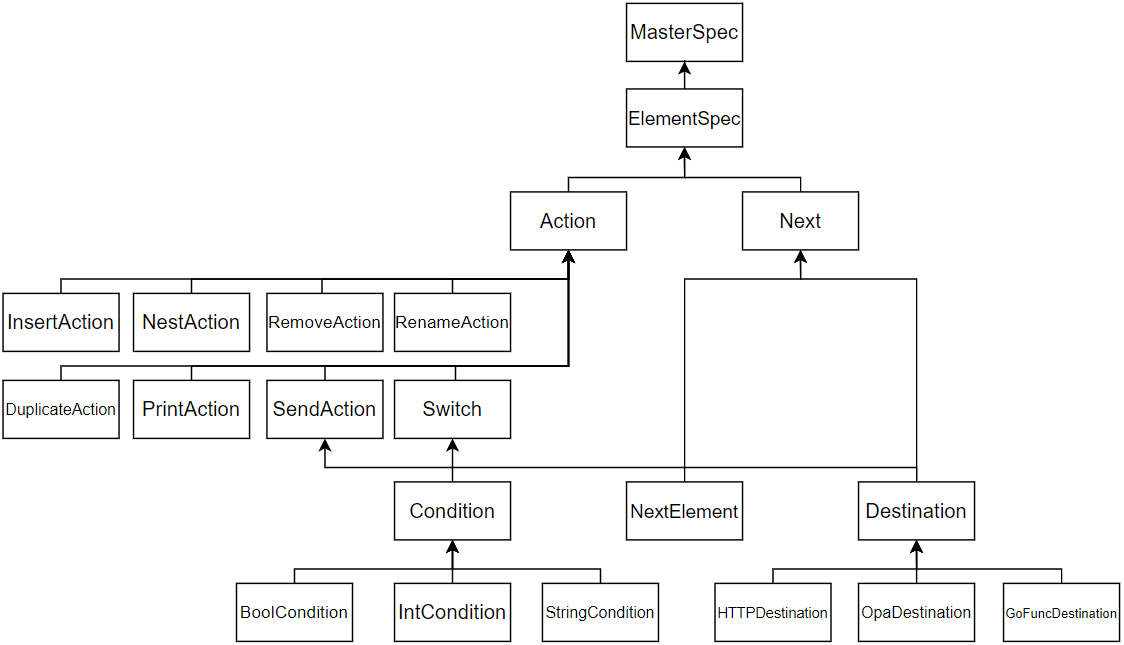
\includegraphics[width=1\linewidth]{a3-tree.png}
    \caption{Drzewko zależności obiektów LupN}\label{fig:a3-tree}
\end{figure}

\subsubsection{MasterSpec}
\begin{lstlisting}[language=go, caption={MasterSpec}\label{lst:a32}]
// MasterSpec defines the desired state of Master
type MasterSpec struct {
	// Name of the Master CR (indicating the name of the loop)
	Name string `json:"name"`
	// Elements is a list of Lupus-Elements
	Elements []*ElementSpec `json:"elements"`
}
\end{lstlisting}
Każdy element na liście \texttt{Elements} spowoduje, że \textbf{Operator Zasobu Master} stworzy obiekt API typu \textbf{Lupus Element}. 

\subsubsection{ElementSpec}
\begin{lstlisting}[language=go, caption={MasterSpec}\label{lst:a32}, basicstyle=\ttfamily\tiny]
// ElementSpec defines the desired state of Element
type ElementSpec struct {
	// Name is the name of the element, its distinct from Kubernetes API Object name, 
    // but rather serves ease of managemenet aspect for loop-designer
	Name string `json:"name"`
	// Descr is the description of the lupus-element, same as Name it serves as 
    // the ease of management aspect for loop-designer
	Descr string `json:"descr"`
	// Actions is a list of Actions that lupus-element has to perform
	Actions []Action `json:"actions,omitempty"`
	// Next is a list of next objects (can be lupus-element or external-element) 
    // to which send the final-data
	Next []Next `json:"next,omitempty"`
	// Name of master element (used as prefix for lupus-element name)
	Master string `json:"master,omitempty"`
}
\end{lstlisting}

\subsubsection{Next}
\begin{lstlisting}[language=go, caption={Next}\label{lst:next}, basicstyle=\ttfamily\tiny]
// Next specifies the next loop-element in a loop workflow, 
// it may be either lupus-element or reference to an external-element
// It allows to forward the whole final-data, but also parts of it
type Next struct {
	// Type specifies the type of next loop-element, lupus-element (element) 
    // or external-element (destination)
	Type string `json:"type" kubebuilder:"validation:Enum=element,destination"`
	// List of input keys (Data fields) that have to be forwarded
	// Pass array with single element '*' to forward the whole input
	Keys []string `json:"keys"`
	// One of the fields below is not null
	Element     *NextElement `json:"element,omitempty" kubebuilder:"validation:Optional"`
	Destination *Destination `json:"destination,omitempty" kubebuilder:"validation:Optional"`
}
\end{lstlisting}

\subsubsection{NextElement}
\begin{lstlisting}[language=go, caption={NextElement}\label{lst:nextelement}]
// NextElement indicates the next loop-element 
// in loop-workflow of type lupus-element
type NextElement struct {
	// Name is the lupus-name of lupus-element 
	// (the one specified in Element struct)
	Name string `json:"name"`
}
\end{lstlisting}

\subsubsection{Destination}
\begin{lstlisting}[language=go, caption={Destination}\label{lst:destination}, basicstyle=\ttfamily\tiny]
// Destination represents an external-element
// It holds all the info needed to make a call to an external-element
// It supports calls to HTTP server, Open Policy Agent or user-functions
type Destination struct {
	// Type specifies if the external element is: a HTTP server in general, 
    // a special kind of HTTP server like Open Policy Agent or internal, a user-function
	Type string `json:"type" kubebuilder:"validation:Enum=http;opa;gofunc"`
	// One of these fields is not null depending on a Type
	HTTP   *HTTPDestination   `json:"http,omitempty" kubebuilder:"validation:Optional"`
	Opa    *OpaDestination    `json:"opa,omitempty" kubebuilder:"validation:Optional"`
	GoFunc *GoFuncDestination `json:"gofunc,omitempty" kubebuilder:"validation:Optional"`
}
\end{lstlisting}

\subsubsection{HTTPDestination}
\begin{lstlisting}[language=go, caption={HTTPDestination}\label{lst:httpdestination}]
// HTTPDestination defines fields specific to a HTTP type
// This is information needed to make a HTTP request
type HTTPDestination struct {
	// Path specifies HTTP URI
	Path string `json:"path"`
	// Method specifies HTTP method
	Method string `json:"method"`
}
\end{lstlisting}

\subsubsection{OpaDestination}
\begin{lstlisting}[language=go, caption={OpaDestination}\label{lst:opadestination}]
// OpaDestination defines fields specific to Open Policy Agent type
// This is information needed to make an Open Policy Agent request
// Call to Opa is actually a special type of HTTP call
type OpaDestination struct {
	// Path specifies HTTP URI, since method is known
	Path string `json:"path"`
}
\end{lstlisting}

\subsubsection{GoFuncDestination}
\begin{lstlisting}[language=go, caption={GoFuncDestination}\label{lst:gofuncdestination}]
// GoFuncDestination defines fields specific to GoFunc type
// This is information needed to call an user-function
type GoFuncDestination struct {
	// Name specifies the name of the function
	Name string `json:"name"`
}
\end{lstlisting}

\subsubsection{Action}
\begin{lstlisting}[language=go, caption={Action}\label{lst:action}, basicstyle=\ttfamily\tiny]
// Action represents operation that is performed on Data
// Action is used in Element spec. Element has a list of Actions 
// and executes them in a workflow manner
// In general, each action has an input and output keys that define 
// which Data fields it has to work on
// Each action indicates the name of the next Action in Action Chain
// There is special type - Switch. Actually, it does not perform any operation on Data, 
// but rather controls the flow of Actions chain
type Action struct {
	// Name of the Action, it is for designer to ease the management of the Loop
	Name string `json:"name"`
	// Type of Action
	Type string `json:"type" kubebuilder:"validation:Enum=send,nest,remove,rename,duplicate,print,insert,switch"`
	// One of these fields is not null depending on a Type.
	Send      *SendAction      `json:"send,omitempty" kubebuilder:"validation:Optional"`
	Nest      *NestAction      `json:"nest,omitempty" kubebuilder:"validation:Optional"`
	Remove    *RemoveAction    `json:"remove,omitempty" kubebuilder:"validation:Optional"`
	Rename    *RenameAction    `json:"rename,omitempty" kubebuilder:"validation:Optional"`
	Duplicate *DuplicateAction `json:"duplicate,omitempty" kubebuilder:"validation:Optional"`
	Print     *PrintAction     `json:"print,omitempty" kubebuilder:"validation:Optional"`
	Insert    *InsertAction    `json:"insert,omitempty" kubebuilder:"validation:Optional"`
	Switch    *Switch          `json:"switch,omitempty" kubebuilder:"validation:Optional"`
	// Next is the name of the next action to execute, in the case of Switch-type action it stands as a default branch
	Next string `json:"next"`
}
\end{lstlisting}

Pole \texttt{Next}, oprócz nazw akcji, może przyjąć jedną z dwóch zdefiniowanych wartości. Wartość \texttt{final} oznacza, że postać \hyperlink{def:dane}{\textbf{Danych}} po tej akcji jest już w swojej \hyperlink{def:finalne-dane}{\textbf{Finalnej Postaci}} i musi zostać przekazana do następnego \hyperlink{def:element-lupus}{\textbf{Elementu Lupus}}. Wartość \texttt{exit} oznacza nagłe zaniechanie aktualnej iteracji \hyperlink{def:zamknieta-petla-sterowania}{\textbf{Pętli Sterowania}} (zazwyczaj wskutek błędu).

\subsubsection{SendAction}
\begin{lstlisting}[language=go, caption={SendAction}\label{lst:sendaction}]
// SendAction is used to make call to external-element
// Element's controller obtains a data field using InputKey,
// and attaches it as a json body when performing a call to destination.
// Response is saved in data under an OutputKey
type SendAction struct {
	InputKey    string      `json:"inputKey"`
	Destination Destination `json:"destination"`
	OutputKey   string      `json:"outputKey"`
}
\end{lstlisting}

\subsubsection{InsertAction}
\begin{lstlisting}[language=go, caption={InsertAction}\label{lst:insertaction}]
// InsertAction is used to make a new field and insert value to it
// Normally new fields are created as an outcome of other types of actions
// It is useful in debugging or logging, 
// e.g. can indicate the path taken by the actions workflow
type InsertAction struct {
	OutputKey string               `json:"outputKey"`
	Value     runtime.RawExtension `json:"value"`
}
\end{lstlisting}

\subsubsection{NestAction}
\begin{lstlisting}[language=go, caption={NestAction}\label{lst:nestaction}]
// NestAction is used to group a number of data-fields together.
// Element's controllers gather fields indicated by InputKeys list
// and nest them in a new field under an OutputKey.
type NestAction struct {
	InputKeys []string `json:"inputKeys"`
	OutputKey string   `json:"outputKey"`
}
\end{lstlisting}

\subsubsection{RemoveAction}
\begin{lstlisting}[language=go, caption={RemoveAction}\label{lst:removeaction}]
// RemoveAction is used to delete a data-field.
// Elements' controllers remove fields indicated by the list InputKeys
type RemoveAction struct {
	InputKeys []string `json:"inputKeys"`
}
\end{lstlisting}

\subsubsection{RenameAction}
\begin{lstlisting}[language=go, caption={RenameAction}\label{lst:renameaction}]
// RenameAction is used to change the name of a data-field.
// InputKey indicates a field to be renamed
// OutputKey is the new field name.
type RenameAction struct {
	InputKey  string `json:"inputKey"`
	OutputKey string `json:"outputKey"`
}
\end{lstlisting}

\subsubsection{DuplicateAction}
\begin{lstlisting}[language=go, caption={DuplicateAction}\label{lst:duplicateaction}]
// DuplicateAction is used to make a copy of a data-field.
// InputKey indicates the field of which value has to be copied.
// OutputKey indicates the field to which values have to be pasted in.
type DuplicateAction struct {
	InputKey  string `json:"inputKey"`
	OutputKey string `json:"outputKey"`
}
\end{lstlisting}

\subsubsection{PrintAction}
\begin{lstlisting}[language=go, caption={PrintAction}\label{lst:printaction}]
// PrintAction is used to print the value of each field 
// indicated by InputKeys in a controller's console.
// It is useful in debugging or logging.
type PrintAction struct {
	InputKeys []string `json:"inputKeys"`
}
\end{lstlisting}

\subsubsection{Switch}
\begin{lstlisting}[language=go, caption={Switch}\label{lst:switch}]
// Switch is a special type of action used for flow-control
// When Element's controller encounters switch action on the chain
// it emulates the work of a switch known in other programming languages
type Switch struct {
	Conditions []Condition `json:"conditions"`
}
\end{lstlisting}

\subsubsection{Condition}
\begin{lstlisting}[language=go, caption={Condition}\label{lst:condition}, basicstyle=\ttfamily\tiny]
// Condition represents a single condition present in Switch action
// It defines on which Data field it has to be performed, 
// the actual condition to be evaluated,
// and the next Action if evaluation returns true.
type Condition struct {
	// Key indicates the Data field that has to be retrieved
	Key string `json:"key"`
	// Operator defines the comparison operation, e.g. eq, ne, gt, lt
	Operator string `json:"operator" kubebuilder:"validation:Enum=eq,ne,gt,lt"`
	// Type specifies the type of the value: string, int, float, bool
	Type string `json:"type" kubebuilder:"validation:Enum=string,int,float,bool"`
	// One of these fields is not null depending on a Type.
	BoolCondition   *BoolCondition   `json:"bool,omitempty" kubebuilder:"validation:Optional"`
	IntCondition    *IntCondition    `json:"int,omitempty" kubebuilder:"validation:Optional"`
	StringCondition *StringCondition `json:"string,omitempty" kubebuilder:"validation:Optional"`
	// Next specifies the name of the next action to execute if evaluation returns true
	Next string `json:"next"`
}
\end{lstlisting}

\subsubsection{BoolCondition}
\begin{lstlisting}[language=go, caption={BoolCondition}\label{lst:boolcondition}]
// BoolCondition defines a boolean-specific condition
type BoolCondition struct {
	Value bool `json:"value"`
}
\end{lstlisting}

\subsubsection{IntCondition}
\begin{lstlisting}[language=go, caption={IntCondition}\label{lst:intcondition}]
// IntCondition defines an integer-specific condition
type IntCondition struct {
	Value int `json:"value"`
}
\end{lstlisting}

\subsubsection{StringCondition}
\begin{lstlisting}[language=go, caption={StringCondition}\label{lst:stringcondition}]
// StringCondition defines a string-specific condition
type StringCondition struct {
	Value string `json:"value"`
}
\end{lstlisting}
